\section{Quicksort}

\textbf{Quicksort} ist ein \textbf{nicht stabiler}, auf Schlüsselvergleichen basierender Sortieralgorithmus, der \textbf{in place} sortiert.

\subsection{Methode}

\textbf{Quicksort} nutzt \textbf{divide-and-conquer}, um ein Feld zu sortieren.\\
Die wesentliche Arbeit erfolgt hier in den Partitionierungs-Schritten, im Gegensatz zu \textbf{Merge-Sort}, hier findet die eigentliche Arbeit im Merge-Schritt statt (vgl.~\cite[174]{GD18e}).\\

\noindent
Bei Quicksort  wird ein Schlüssel aus dem Feld als \textbf{Pivot-Element} $p$ gewählt (im folgenden immer das rechte einer Teilfolge).\\
Alle Schlüssel, die kleiner als das Pivotelement sind, werden in die eine Hälfte geschrieben, alle die größer sind, in die andere.
Das Pivotelement selber wird zwischen die beiden Hälften geschrieben, die dann durch Rekursion wiederholt bearbeitet werden, bis die Teilfelder die Größe $1$ haben, womit das gesamte Feld als sortiert gilt:\\
Zwei Positionszeiger $i$ und $j$ wandern symmetrisch von links nach rechts ($i$) bzw. rechts nach links ($j$) in der Folge, bis ein Schlüssel $k_i > p$ und $k_j < p$ gefunden wurde. \\
Die Schlüssel an Position $i$ und $j$ werden dann miteinander getauscht.\\
Kreuzen sich $i$ und $j$, gilt für alle Schlüssel $k_u < p$ (mit $u < i$ ), und für alle Schlüssel $k_v > p$ (mit $v > j$)).
In dem Fall wird der Schlüssel an Position $i$ mit dem Pivotelement $p$ getauscht, und das Feld wird an dieser Stelle in zwei Teilfolgen aufgeteilt, wonach die Prozedur für die entstandenen Teilfolgen wiederholt wird (s. Abbildung~\ref{fig:quicksort}).

\subsection{Implementierung}

\begin{minted}{java}
    quicksort (int[] arr, int l, int r) {
        if (l >= r) {
            return;
        }
        int i = l;
        int j = r - 1;
        int pivot = arr[r];
        while (i <= j) {
            while (i < r && arr[i] <= pivot) {
                i++;
            }
            while (j >= 0 && arr[j] > pivot) {
                j--;
            }
            if (i < j) {
                int tmp = arr[i];
                arr[i] = arr[j];
                arr[j] = tmp;
            }
        }
        arr[r] = arr[i];
        arr[i] = pivot;

        quicksort(arr, l, i - 1);
        quicksort(arr, i + 1, r);
    }
\end{minted}

\begin{figure}
    \begin{center}
        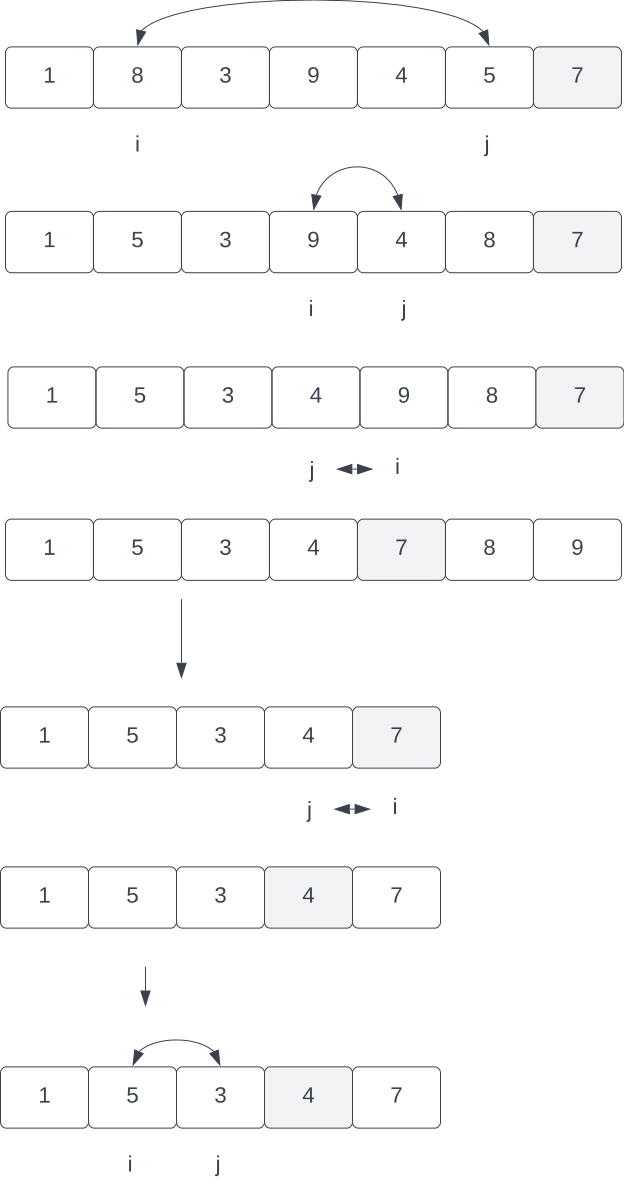
\includegraphics[scale=0.3]{chapters/Sortierverfahren/img/quicksort1}
    \end{center}
    \begin{center}
        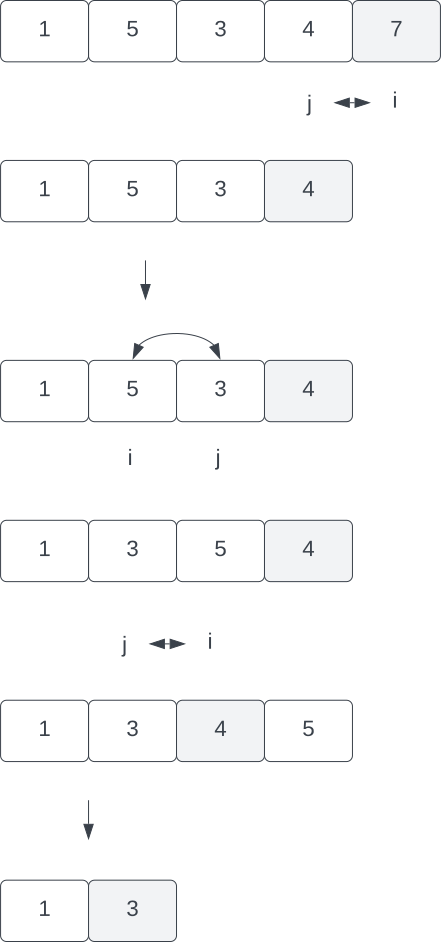
\includegraphics[scale=0.3]{chapters/Sortierverfahren/img/quicksort2}
        \caption{Anwendung von Quicksort auf das Feld $1,\ 8,\ 3,\ 9,\ 4,\ 5,\ 7$. Das Pivotelement ist jeweils hervorgehoben. Sobald sich $i$ und $j$ kreuzen, findet eine Partitionierung der Folge statt, und die Methode wird rekursiv auf die Teilfolgen angewendet. Nicht dargestellt sind bereits vollständig sortierte Teilfolgen. (Quelle: eigene)}
        \label{fig:quicksort}
    \end{center}
\end{figure}


\subsection{Laufzeit}
Im \textbf{worst-case} hat Quicksort eine Laufzeit von $O(n^2)$, allerdings wird in der Literatur darauf hingewiesen, dass das Sortierverfahren eins der schnellsten Sortierverfahren ist, da es im Mittel mit $O(n\ log\ n)$ sortiert (vgl.~\cite[92]{OW17b} sowie ~\cite[173]{GD18e}).\\
\textit{Güting und Dieker} weisen in~\cite[182 f.]{GD18e} darauf hin, dass die \textbf{Effizienz} von Quicksort im Wesentlichen von der Wahl des Pivot-Elementes als auch von der \textit{Rekursionstiefe} abhängt.